\chapter{Numerical Values and Quantization Errors}\label{ch:numbers}

Human brains understand conceptually continuous quantities such as real numbers as well as discrete quantities such as integers and characters.  On the other hand, if you are asked to write down a continuous number explicitly, you quickly realize that it is not possible. For example, we cannot write down the exact value of $\pi$ as a string of numbers.  We can write it only approximately like 3.14. When we calculate mathematical expressions symbolically, we don't have to worry about errors caused by such approximation..  However, when we calculate numerically, we use such approximation unless the number is integer or exact fraction.  The situation is similar to hand calculation we do regularly. When we carry out a lengthy calculation, we often write down intermediate values temporarily on the back of envelope with only finite figures and use them at a later time.  They are not exact numbers but we hope accurate enough in practice. The current digital computers work essentially in the same manner. 
We must keep it in our mind that digital computers can understand only very limited numbers as we discuss in this chapter. We have to ask computers only what they can understand. When we force computers to do something beyond their capabilities, they often pretend that they understood it and give us an answer, but a wrong one.  At present computers are not smart enough to tell what they can do and what they cannot do.  Therefore, we first need to understand how the digital computers handle numerical quantities and their limitation.
 
\section{Bits}

The current digital computers are mostly binary machines\footnote{We don't consider q-bit used in quantum computers.} and use a bit $b$ as the smallest unit of information where $b=0$ or $1$ (or we write it equivalently as $b=\{0,1\}$). Inside a computer,  information is generally encoded in a string of bits such as $01100101000101100\cdots$.  The number of unique expressions depends on the length of the string, which is measured as the number of bits. An $N$-bit string
\[
N\text{-bit string} = b_{N-1} b_{N-2} \cdots b_2 b_1 b_0
\]
can express $2^N$ different values.  For instance, there are only four possible realizations of a 2-bit string: 00, 01, 10, 11.  $N$ can be very large but always finite and limited by the size of hardware.\footnote{Our brain also consists of a finite number of neurons but it is huge (about $10^{11}$). Despite of that, humans are able to develop the concept of infinity and continuous numbers!}
The common lengths of the binary string in the present computers are 8, 16, 32, and 64.   The string of 8 bit is called a byte.  The number of different expressions these strings can have is shown in Table \ref{tbl:binary-sizes}.

\begin{table}[tb]
\centering
\caption{Common binary strings and their capacity}\label{tbl:binary-sizes}
\begin{tabular}{ccl}
Size in bits & Size in bytes & number of different expressions\\
\hline
 8  & 1 & $2^8$=256 \\
16  & 2 & $2^{16}$=65536\\
32  & 4 & $2^{32}$=4,294,967,296\\
64  & 8 & $2^{64}$=18,446,744,073,709,551,616\\
\hline
\end{tabular}
\end{table}


We \textit{encode} numbers and characters in binary strings and \textit{decode} binary strings to get human-readable information.  Encoding/decoding is not a one-to-one map.
The same one byte of string may correspond to multiple different things, integer, character, and others as shown in the following sections.  Some computer languages (dynamical language) choose an appropriate encoding scheme based on the context but in compiler-based languages, programmers must declare the type of quantity before using it or otherwise computer issues an error message.


\noindent
\section{Integers}\label{sec:integer}

Since integers are discrete and exact enumeration is possible, computers usually treat integers differently from continuous numbers.  That means 1 and "1.0" are expressed in different binary strings.  Encoding integers are relatively simple. If an integer
expressed in binary form
\[
I = \sum_{k=0}^{N-1} 2^k b_k
\]
then the corresponding binary string 
\[
[b_{N-1} \cdots b_2 b_1 b_0]
\]
For example, binary number $101$ corresponds to integer $1\times 1+ 2 \times 0 + 4 \times 1 =5$.   Noting that an 8-bit binary string can express $256$ different integers, it can express integers from 0 to 255. In general, an $N$-bit string encodes integers from 0 to $2^N-1$.  Since negative integer is not included, this type of integer is called \textit{unsigned integer}.

If a \textit{signed integer} is needed, one bit of the binary string is used to specifies the sign, 0 for $+$ and 1 for $-$, and remaining bits are used for the magnitude. An 8-bit binary string spans from $-128$ to $+127$.  Table \ref{tbl:int_range} shows the range of other integer types.  The default size of signed integer is 32 bit in most computer languages.  However, 64-bit integer is used for large scale calculation.  Mots common CPUs cannot handle integer larger than 64 bit.  If more than 64 bit is needed, you must use a special numerical library.

\begin{table}[tb]
\centering
\caption{The range of unsigned and signed integers in \texttt{MATLAB}}
\label{tbl:int_range}
\begin{tabular}{c|rr|rr }
\hline
& \multicolumn{2}{|c}{unsigned} & \multicolumn{2}{|c}{signed} \\
\cline{2-5}
\raisebox{6pt}{bits} & min & max & min & max \\
 \hline
8 & 0 & 255 & -128 & +127 \\
16 & 0 & 65535 & -32768 & +32767 \\
32 & 0 & 4294967295 & -2147483648 & +2147483647\\
64 & 0 & 18446744073709551615 & -9223372036854775808
& 9223372036854775807 \\
\hline
\end{tabular}
\end{table}

\texttt{MATLAB} has 4 classes of unsigned integer, \texttt{uint8},
\texttt{uint16},  \texttt{uint32}, and  \texttt{uint64}.  Similarly, there are 4 classes of signed integer, \texttt{int8},
\texttt{int16},  \texttt{int32}, and  \texttt{int64}.
Functions \texttt{intmax()} and \texttt{intmin()} return the smallest and largest integer values for a specified class. See Example \ref{ex:minmaxint}.  

\noindent
\begin{example}[Maximum and minimum of integers]\label{ex:minmaxint}
\small
\begin{mybox}
\begin{verbatim}
>> intmax('int16')
ans =
      32767
>> intmin('int16')
ans =
     -32768
\end{verbatim}
\end{mybox}
\normalsize
\end{example}

\noindent
\exercise
Verify the data given in Table \ref{tbl:int_range} using \texttt{intmax} and \texttt{intmin}.

\bigskip
If you don't remember the type of variable, you can use MATLAB function \texttt{class()} to find it out.
In MATLAB the default type is real64.

\noindent
\begin{example}[Identify the type]\label{ex:minmaxint}
\small
\begin{mybox}
\begin{verbatim}
>> y=int32(2);
>> class(y)
ans =
      int32
\end{verbatim}
\end{mybox}
\normalsize
\end{example}

\bigskip

\noindent
\section{Characters}\label{sec:characters}


In English or most of western languages, the number of alphanumeric characters is less than $256$.  Hence, all characters can be encoded in one byte ($8$-bit) binary string.  In US, the encoding map is known as ASCII  (American Standard Code for Information Interchange)\cite{wiki_ascii} and lower and upper cases of all letters and various symbols are encoded in 7-bit strings.  For example, 'A'=1000001B and 'a'=1100001B. (B at the end indicates that the string is a binary code.)  Note that integer 1=00000001B and character '1'=00110001B in ASCII are two different things.  Sending 00000001B to a printer does not print 1.  You need to convert number to character string. When you type  '1' on a keyboard, you are sending character '1' to computer.  You need to convert it to integer. I/O functions do that automatically.  If you want to convert manually, use \texttt{num2str()} and \texttt{str2num}.  See Example \ref{ex:num2str}.

Some languages use a lot more characters than $256$.  For example, Chinese uses a few thousand characters.  Therefore, $8$-bit string is not large enough. Two-byte ($16$-bit) strings can encode $65536$ characters, which seems long enough for all languages.

\begin{example}[Character-number conversion]\label{ex:num2str}
\small
\begin{mybox}
	\begin{verbatim}
>> num2str(12)
ans =
      '12'
>> str2num('12')
ans =
      12
\end{verbatim}
\end{mybox}
\normalsize
\end{example}

\noindent
\section{Floating Point Numbers}\label{sec:float}

There is no way to express real numbers in discrete systems. For example, we cannot express any irrational number using a finite number of letters 0-9.  Therefore, we express real number approximately using scientific notation such as $1.32567 \times 10^{12}$.  Similarly digital computers use so-called \emph{floating point} representation.  A \emph{single precision} floating point stores a real number in a 32-bit string, of which 24 bits are used for mantissa.  The corresponding significant figure is $\log_{10} 2^{24} \approx 7$.  The exponent part is $2^{2^7}=2^{-128}$ to $2^{2^7-1}=2^{127}$ which is approximately $10^{-38}$ to $10^{+38}$.  Usually, the single precision is not accurate enough for computational physics. A double precision floating point uses a 64-bit string, 54 bits for mantissa and 10 bits for exponent.  The largest value the mantissa can express  is $2^{53} = 9007,199,254,740,992$, which corresponds to significant figure 16.  The maximum exponent part is between $2^{-2^9} = 2^{-512} \approx 10^{-308}$ and $2^{2^9-1} = 2^{511} \approx 10^{308}$.\footnote{The actual smallest value in many languages is $4.9406564584124654 \times 10^{-324}$ for double and $1.401298 \times 10^{-45}$ for single because there is a better way (denormalized float) to handle small values.  We do not discuss it here.}   Floating point encoding uses two different zeros, $-0 \ne +0$.

Since the floating point numbers are \emph{quantized}, there is always a gap between the nearest two floating point numbers.  Any values inside the gap cannot be expressed in standard computer languages, which may causes inaccurate results due to quantization error.\cite{widrow2008}  The positive value next to zero is $1.1754944 \times 10^{-38}$ for single precision.  If we try to use a number between zero and the smallest floating point value, \textit{underflow} error occurs.   We will discuss it in the next section. 

Another gap we should pay attention to is the machine epsilon $\epsilon$, the gap between 1 and next number $1+\epsilon$ (see Fig. \ref{fig:machine_epsilon}).  We will write a code to find the machine epsilon in the later section.

Some of floating point values are assigned to special meaning $\pm$\texttt{Inf} = $\pm \infty$ and \texttt{NaN} = "Not a Number". See Example \ref{ex:InfNaN}.


\bigskip
\begin{example}[Range of floating point numbers]
\small
\begin{mybox}
	\begin{verbatim}
% Print the smallest and largest double precision value.
>> fprintf('%25.16e, %25.16e\n',realmin(),realmax());   
  2.2250738585072014e-308,   1.7976931348623157e+308
\end{verbatim}
\end{mybox}
\normalsize
\end{example}

\noindent
\exercise\label{ex:minmaxfloat}
Find the largest and smallest values of single precision floating point numbers.
\vspace{18px}

\begin{figure}[tb]
\centering
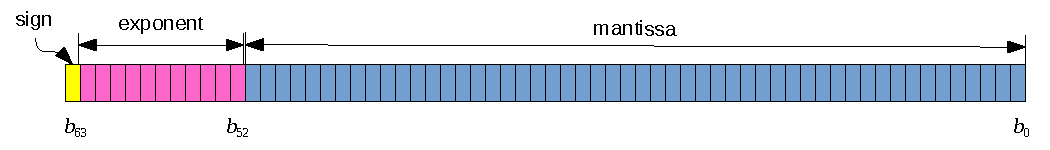
\includegraphics[width=5.5in]{01.numbers/double-float.pdf}\label{fig:double-float}
\caption{64-bit string for floating point expression.  The last bit is used for the sign and 11 bits from $b_{52}$ to $b_{62}$ express the exponent.  The remaining 52 bits express the mantissa.}
\end{figure}

\begin{figure}[tb]
\centering
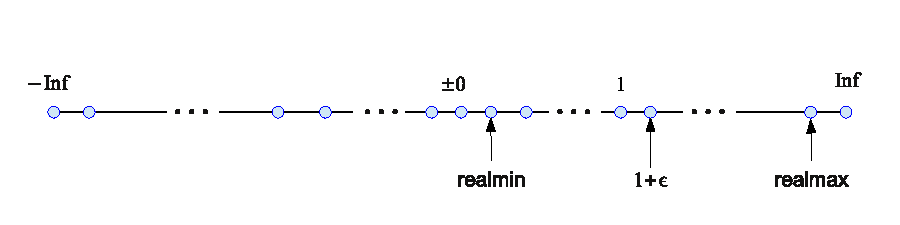
\includegraphics{01.numbers/floating-point-line.pdf}
\caption{Discreteness of floating point numbers. $\epsilon$ is the machine epsilon discussed in Sec. \ref{sec:epsilon}.}
\label{fig:machine_epsilon}
\end{figure}

\begin{example}[Special floating point numbers, Inf and NaN]\label{ex:InfNaN}
	
Anyhing bigger than \texttt{realmax} is \texttt{Inf} ("infinity") in the computer world.  Undefined number such as 0/0 is \texttt{NaN} ("Not a Number").
\small
\begin{mybox}
	\begin{verbatim}
>> realmax * 10
ans =
      Inf    
>> 0/0
ans =
      NaN
\end{verbatim}
\end{mybox}
\normalsize
\end{example}

\noindent
\exercise
Evaluate $1/0$ and $1/$\texttt{Inf}.  Are the outputs consistent with common mathematics?
\vspace{18px}

\noindent
\section{Overflow/Underflow}\label{sec:overflow}
If we try to use a value bigger than the computer can understand, what will happen? 
It results in \emph{Overflow error}.  For example, if you try to store $1.0 \times 10^{60}$ into a single precision floating point variable, the value is replaced by Inf.  Similarly, if the value is too small, it is replaced with 0.  For example, $1.0 \times  10^{-60}$ is too small for a single precision floating point. The zero may cause a problem later such as divided by zero.

In most cases, we can avoid the range errors at least for physics problems.
Many quantities have dimension and their values depend on the choice of units. Fortunately, dimensionless constants in physics are usually order of 1 or close to it. Therefore, we can avoid the range error using appropriate units.
However, there are problems which contain intrinsically large numbers without units.  For example, in statistical mechanics we often evaluate $N!$ where $N$=number particles at the order of Avogadro constant $N_A=6.02214129 \times 10^{23}$.  There is no way to compute $N!$ directly.  Even then there are tricks to calculate such large values (with help of mathematics).

We can avoid the range error in the following ways:

\begin{center}
\begin{minipage}{5in}
\begin{itemize}
\item[1.] Change the order of calculation so that large values do not appear during the calculation.
\item[2.] Use different units so that numbers are not very large or small.
For example, if \textit{atomic unit} is used, $\hbar=e=m=1$, and $\epsilon_0 = \frac{1}{4\pi}$.  The Bohr radius is simply $a_0=1$!.  In the atomic world, it is better to measure distance using the radius of hydrogen atom as a unit.  See Example \ref{ex:bohr_radius} for the calculation of $a_0$ in SI units.
\item[3.] If $x$ is too large, evaluate $y=\ln(x)$.   Then, $x=e^y$ or if base 10 is used, $x=10^y$. See Example \ref{ex:factorial}.
\end{itemize}
\end{minipage}
\end{center}

\begin{example}[Evaluation of Bohr radius]
    \label{ex:bohr_radius}
\medskip
Evaluate the Bohr radius (the radius of a hydrogen atom)\cite{Griffiths} in SI unit.    The Bohr radius is given by
$a_0 = \displaystyle\frac{4 \pi \epsilon_0 \hbar^2}{m e^2}$ where
\begin{eqnarray*}
\epsilon_0\, (\text{vacuum permittivity}) &=& 8.854187817 \times 10^{-12} F/m\\
\hbar\, (\text{Planck constant}) &=& 6.62606957 \times 10^{-34}/2\pi, m^2\, kg / s \\
m\, (\text{electron mass}) &=& 9.10938291 \times 10^{-31}\, kg\\
e\, (\text{elementary charge}) &=& 1.602176565 \times 10^{-19} C
\end{eqnarray*}

If you evaluate the numerator and denominator independently, each values may cause overflow error. By grouping the numbers in an appropriate way, you can avoid the overflow error.

\small
\begin{mybox}
\begin{verbatim}
>> epsilon=single(8.854187817e-12);
>> hbar=single(6.62606957e-34/(2*pi));
>> mass=single(9.10938291e-31);
>> e=single(1.602176565e-19);
>> a=4*pi*epsilon*hbar^2/(mass*e^2)
a =
     NaN

>> a=4*pi*(epsilon/mass)*(hbar/e)^2
a =
    5.2918e-11
\end{verbatim}
\end{mybox}
\normalsize
\end{example}

\noindent
\exercise
Evaluate the Bohr radius using double precision.  Confirm that even the dumb method causing the range error in the example is OK with double precision.
\vspace{18px}

\begin{example}[Factorial of large number]\label{ex:factorial}
Factorial of a large integer is astronomically large.  It is obviously an integer but too long to write it down.  For example, 1000! is as long as
\tiny
\begin{mybox}
\begin{verbatim}
4023872600770937735437024339230039857193748642107146325437999104299385123986290205920442084869694048004799886101971960586316668729948085589013238
2966994459099742450408707375991882362772718873251977950595099527612087497546249704360141827809464649629105639388743788648733711918104582578364784
9977012476632889835955735432513185323958463075557409114262417474349347553428646576611667797396668820291207379143853719588249808126867838374559731
7461360853795345242215865932019280908782973084313928444032812315586110369768013573042161687476096758713483120254785893207671691324484262361314125
0878020800026168315102734182797770478463586817016436502415369139828126481021309276124489635992870511496497541990934222156683257208082133318611681
1553615836546984046708975602900950537616475847728421889679646244945160765353408198901385442487984959953319101723355556602139450399736280750137837
6153071277619268490343526252000158885351473316117021039681759215109077880193931781141945452572238655414610628921879602238389714760885062768629671
4667469756291123408243920816015378088989396451826324367161676217916890977991190375403127462228998800519544441428201218736174599264295658174662830
2955570299024324153181617210465832036786906117260158783520751516284225540265170483304226143974286933061690897968482590125458327168226458066526769
9586526822728070757813918581788896522081643483448259932660433676601769996128318607883861502794659551311565520360939881806121385586003014356945272
2420634463179746059468257310379008402443243846565724501440282188525247093519062092902313649327349756551395872055965422874977401141334696271542284
5862377387538230483865688976461927383814900140767310446640259899490222221765904339901886018566526485061799702356193897017860040811889729918311021
1712298459016419210688843871218556461249607987229085192968193723886426148396573822911231250241866493531439701374285319266498753372189406942814341
1852015801412334482801505139969429015348307764456909907315243327828826986460278986432113908350621709500259738986355427719674282224875758676575234
4220207573630569498825087968928162753848863396909959826280956121450994871701244516461260379029309120889086942028510640182154399457156805941872748
9980942547421735824010636774045957417851608292301353580818400969963725242305608559037006242712434169090041536901059339838357779394109700277534720
0000000000000000000000000000000000000000000000000000000000000000000000000000000000000000000000000000000000000000000000000000000000000000000000000
0000000000000000000000000000000000000000000000000000000000000000000000000000000000000000000000000000000
\end{verbatim}
\end{mybox}
\normalsize

which is practically useless.  In fact, MATLAB retuns \texttt{Inf} for 1000!.
Therefore, we want to write it approximately in scientific notation  $a \times 10^{b}$.

In order to find the mantissa $a$ and exponent $b$, first we evaluate $\log N!$ as follows.
\begin{eqnarray}
y&=&\log(N!) = \log(1 \cdot 2 \cdot 3 \cdots N-1 \cdot N) \nonumber \\
&=& \log(1)+\log(2)+\log(3)+\cdots + \log(N-1)+\log(N)
\end{eqnarray}
Once you found $y$, $n! = e^y$.  However, it is still not in scientific notation.  First we change the base from $e$ to $10$ as $e^y  = 10^z $,  where $z = y \log_{10}(e)$.  Then, $n! = 10^z$.
Next we split $z$ to the floor k=$\lfloor z \rfloor$ and the residual $\delta=z - \lfloor z \rfloor$.
Now, we have $n! = 10^{k+\delta} = 10^\delta \times 10^k$ and thus the mantissa is $10^\delta$ and power is $k$.  Using this method, $1000! \approx 4.0239 \times 10^{2567}$. The mantissa and the power are obtained in the following way.

\bigskip
\small
\begin{mybox}
	\begin{verbatim}
>> factorial(1000)
ans =
   Inf

>> y=sum(log(1:1000))
y =
   5.9121e+03

>> z=log10(exp(1))*y
z =
   2.5676e+03
   
>> power=floor(z)
power =
    2567
    
>> mantissa=10^(z-power)
mantissa =
    4.0239
   \end{verbatim}
\end{mybox}
\normalsize
\end{example}

\noindent
\exercise
Express $10000!$ in scientific notation.

\bigskip
\noindent
\section{Machine Epsilon}\label{sec:epsilon}

Although a double precision number covers from a small number $2.2250738585072014\times 10^{-308}$ to a large number $1.7976931348623157 \times 10^{+308}$, it can distinguish only 18446744073709551616 values.  There is a gap between two closest floating point numbers.  A floating point number next to 1 is $1+\epsilon$ where $\epsilon$ is called \emph{machine epsilon}, whose value depends on the systems.  If you add a half of $\epsilon$ to 1, there is no floating point expression to the answer.  So what will happen if you try to calculate $1+\displaystyle\frac{\epsilon}{2}$. The computer thinks $1+\displaystyle\frac{\epsilon}{2} = 1$.  In the following example, you can find the machine epsilon of your computer.

\bigskip
\begin{example}[Machine epsilon built in computer language]

Most of computer languages have a function which returns the value of machine epsilon.  
Confirm that $1+\frac{\epsilon}{2} = 1$ using MATLAB command \texttt{eps()}.

\small
\begin{mybox}
	\begin{verbatim}
>> fprintf('%25.16e\n%25.16e\n%25.16e\n', eps(), 1+eps(), 1+eps()/2);
2.2204460492503131e-16
1.0000000000000002e+00
1.0000000000000000e+00
   \end{verbatim}
\end{mybox}
\normalsize
\end{example}

\bigskip
\begin{example}[Machine epsilon appears even in a simple arithmetic calculation]
	
It is easy to see that  $\displaystyle\frac{5}{3}-\frac{2}{3}-1$ and $\displaystyle\frac{7}{3}-\frac{4}{3}-1$ are both exactly zero.  However, computers don't think so.  The former vanishes as expected but the latter equals to the machine epsilon.
\small
\begin{mybox}
	\begin{verbatim}]
>> 5/3-2/3-1
ans = 0
>> 7/3-4/3-1
ans = 2.2204e-16
   \end{verbatim}
\end{mybox}
\normalsize
\end{example}

	
\bigskip
\begin{example}[Finding machine epsilon]
To find  machine epsilon, we check if $1+2^{-n}$ is bigger than $1$ for positive integer $n$.  As $n$ increases, $2^{-n}$ gets smaller and smaller.  At a certain value of $n$, it becomes too small and computer thinks $1+2^{-n} = 1$.  Then, the machine epsilon is $\epsilon = 2^{-(n-1)}$.  Program \ref{matlab:machine_epsilon}\footnote{Example codes are listed at the end of each chapter.} finds the machine epsilon using this method.  The output is 
\small
\begin{mybox}
	\begin{verbatim}
32 bit floating point
Stopped after  24 iterations 
machine epsilon by computation =    1.1920929e-07 
machine epsilon by MATLAB      =    1.1920929e-07 
1 + epsilon   =   1.00000012e+00 
1 + epsilon/2 =   1.00000000e+00 
   \end{verbatim}
\end{mybox}
\normalsize

\noindent
The value agrees with the machine epsilon obtained by MATLAB command \texttt{eps()}.
\end{example}

\noindent
\exercise
Modify Program \ref{matlab:machine_epsilon} and find the machine epsilon for double precision floating point.


\noindent
\section{Round-off Errors}\label{sec:roundoff}

When you apply some operation to two numbers such as addition, the resulting number may not exist in floating point expression.  The machine picks a nearest number.
Therefore, every operation induces some error called round-off error.  Such an error is small but accumulates over many operations and significant figures decreases after many operations. Such an error causes a fatal error when you subtract a number from a very similar number.  Suppose that two single floating point numbers have exactly the same first 5 digits.  The last two digits are not reliable due to the round-off error.  Now you subtract one from the other, only the last two digits remain in the outcome. Therefore, the outcome is not reliable at all.  You must avoid the such subtraction.

The round-off error is an serious issue for digital computers.  On February 25, 1991, during the Gulf War, an American Patriot Missile battery in Dharan, Saudi Arabia, failed to track and intercept an incoming Iraqi Scud missile. The Scud struck an American Army barracks, killing 28 soldiers and injuring around 100 other people. Patriot missile.  Round-off error is suspected to have caused this tragedy.\cite{Skeel1992} 

\bigskip
\begin{example}[Accumulation of Round-off Error]
\label{ex:manyadds}
For $x=1.2$, add $x$ 100000 times and compare the result with $100000 \times x$.  Mathematically speaking the two calculation should give the same answer.  See what your computer says.

\small
\begin{mybox}
	\begin{verbatim}
>> x=single(1.2);
>> xsum=single(0);
>>for i=1:100000
xsum=xsum+x;
end
>>xmul=single(100000)*x;
>> fprintf('Iteration=%14.7e,  Multiplication=%14.7e\n',xsum,xmul);
Iteration= 1.2011162e+05,  Multiplication= 1.2000001e+05
   \end{verbatim}
\end{mybox}
\normalsize
\end{example}


\bigskip
\noindent
\exercise
\begin{itemize}
\item[(a)]  Repeat Example \ref{ex:manyadds} with $x=2$.  The error disappears. Why?
\item[(b)]  Repeat Example \ref{ex:manyadds} using double precision.  Do you still see the round-off error?
\end{itemize}

\noindent
\section{Loss of Significance}\label{sec:significance}

Since the floating point expression of real numbers can keep only finite digits, we need to pay attention to the significant figures like we do for hand calculation with approximate numbers.  The error can be very severe particularly when two similar numbers are subtracted from one another (known as \emph{catastrophic cancellation}).  Foe examp,e let us calculate $0.123456789 \times 10^{-5} - 0.123456700 \times 10^{-5}$ using 32-bit floating point.  The exact value is $0.89 \times 10^{-12}$.   Here is the MATLAB output:

\small
\begin{mybox}
	\begin{verbatim}
>> x=single(0.123456789e-5)-single(0.123456700e-5);
>> fprintf('%16.7e',x)
9.0949470e-13
   \end{verbatim}
\end{mybox}
\normalsize
The significant figure is only one. The other digits '949470' has no significance but MATLAB prints them out as if they are a part of the answer.  If you use this number for other calculation, significant figures may be reduces to none.   The number you get may have no significance.  We need to try to avoid subtraction of similar numbers to keep the significant figures.  Note that addition has no such problem.

\begin{example}[Catastrophic cancellation]
\label{ex:twosimilarvalues}
Evaluate $\displaystyle\frac{(x+1)^2-1}{x}$ for $x$ from $10^{-1}$ to $10^{-17}$.
Compare the numerical results with the exact solution, $x+2$, which is always bigger than 2 for positive $x$.  When $x$ is smaller than machine epsilon, computer thinks that $x+1=1$ and thus the result is zero!
\small
\begin{mybox}
Script:

	\begin{verbatim}
for i=1:17
y(i)=((x(i)+1)^2-1)/x(i);
z(i)=x(i)+2;
fprintf('x=%8.1e, direct=%10.7f,  exact= %10.7f\n', x(i),y(i),z(i));
end
   \end{verbatim}

\medskip
Output:
	\begin{verbatim}
x= 1.0e-01, direct= 2.1000000,  exact=  2.1000000
x= 1.0e-02, direct= 2.0100000,  exact=  2.0100000
x= 1.0e-03, direct= 2.0010000,  exact=  2.0010000
x= 1.0e-04, direct= 2.0001000,  exact=  2.0001000
x= 1.0e-05, direct= 2.0000100,  exact=  2.0000100
x= 1.0e-06, direct= 2.0000010,  exact=  2.0000010
x= 1.0e-07, direct= 2.0000001,  exact=  2.0000001
x= 1.0e-08, direct= 2.0000000,  exact=  2.0000000
x= 1.0e-09, direct= 2.0000002,  exact=  2.0000000
x= 1.0e-10, direct= 2.0000001,  exact=  2.0000000
x= 1.0e-11, direct= 2.0000002,  exact=  2.0000000
x= 1.0e-12, direct= 2.0001778,  exact=  2.0000000
x= 1.0e-13, direct= 1.9984015,  exact=  2.0000000
x= 1.0e-14, direct= 1.9984015,  exact=  2.0000000
x= 1.0e-15, direct= 2.2204460,  exact=  2.0000000
x= 1.0e-16, direct= 0.0000000,  exact=  2.0000000
x= 1.0e-17, direct= 0.0000000,  exact=  2.0000000
   \end{verbatim}
\end{mybox}
\normalsize
\end{example} 

\noindent
\exercise
Repeat Exercise \ref{ex:twosimilarvalues} using double precision.  Reduce the value $x$ until the result deviate significantly from the exact value.

\bigskip
\begin{example}[Roots of Quadratic Equation]
	The solutions to quadratic equation $a x^2 + b x + c = 0$ are well-known:
	\begin{subequations}\label{eq:roots-original}
		\begin{equation}
		x_1 = \frac{-b - \sqrt{b^2 - 4 a c}}{2a} \label{eq:root-}
		\end{equation}
		\begin{equation}
		x_2 = \frac{-b + \sqrt{b^2 - 4 a c}}{2a}\label{eq:root+}
		\end{equation}
	\end{subequations}
	For simplicity, we assume $b>0$.
	Solution $x_1$ does not cause a serious round-off error. However, when $b^2 \gg a c$, the other solution  $x2$  involves subtraction of two similar numbers and thus it is vulnerable to catastrophic cancellation. The error is especially severe when $a \ll b$ because the denominator is very small and the situation is close to 0/0. Fortunately, there is a simple way to avoid this loss of significance. Using the equality
	\begin{equation}
	x_2 = \frac{-b + \sqrt{b^2 - 4 a c}}{2a} = \frac{-2c}{b+\sqrt{b^2 - 4 a c}} = \frac{c}{a x_1}
	\label{eq:quad_trick1}
	\end{equation}
	the subtraction causing catastrophic cancellation disappears.  Similarly for $b<0$, Eq. \eqref{eq:root-} which may cause catastrophic cancellation can be evaluated by 
	\begin{equation}
	x_1 = \frac{-b - \sqrt{b^2 - 4 a c}}{2a} = \frac{-2c}{-b+\sqrt{b^2 - 4 a c}} = \frac{c}{a x_2}.
	\label{eq:quad_trick2}
	\end{equation}
	There are many pitfalls with the floating point numbers.  See more examples in Ref. \cite{Goldberg1991}.
	
\bigskip
\begin{myalgobox}
	\Algorithm{Roots of Quadratic Equation}\label{algo:roots-quad}

\bigskip
Roots of $a x^2 + b x + c = 0$ ($a \ne 0$ and $b \ne 0$).
\begin{eqnarray}
x_1 &=& \frac{-b - \text{sgn}(b)\sqrt{b^2 - 4 a c}}{2a} \\
x_2 &=& \frac{c}{a x_1}
\end{eqnarray}
where
\[
\sign(b) = \begin{cases} +1 & b>0 \\ -1 & b<0 \end{cases}
\]
\end{myalgobox}

\end{example}

\bigskip

\noindent
\section*{Problems}
\addcontentsline{toc}{section}{\protect\numberline{}Problems}

\begin{enumerate}[labelwidth=0.5cm,labelindent=0.0cm,leftmargin=*,label=\bfseries \thechapter.\arabic*,align=left]
\item
Evaluate the roots of $a x^2 + x + \displaystyle\frac{1}{4} = 0$ using the original formula Eqs. \eqref{eq:roots-original} and Algorithm \ref{algo:roots-quad}. Reduce the value of $a$ as 0.1, 0.01, 0.001, $\cdots$ until it hits the machine epsilon. Note that the exact answer for $a=0$ is $x=-\displaystyle\frac{1}{4}$.  Observe that the original formula fails but the improved one works.
\item In statistical mechanics, factorial $n!$ of huge integer $n$ such as the Avogadro number often appears. It is difficult to manage such a huge number even analytically.  A common method to deal with such problem is to use the Stirling formula\cite{Zwillinger2012}:
\begin{equation}
\ln(n!) \approx n \ln(n) - n + \frac{1}{2} \ln(2 \pi n)
\label{eq:stirling1}
\end{equation}
Then, the factorial can be approximated by
\begin{equation}
n! \approx \sqrt{2 \pi n} \left ( \frac{n}{\text{e}} \right )^n\, .
\label{eq:stirling2}
\end{equation}
To verify the accuracy of this formula, compute the ratio $R=\displaystyle\frac{n!}{\sqrt{2 \pi n} \left ( \frac{n}{\text{e}} \right )^n}$  for $n=10, 100$, and $1000$.  Verify that formula (\ref{eq:stirling2}) approaches the exact value as $n$ increases. Note that direct calculation of $R$ is hard but $\ln R$ can be easily evaluated.
\end{enumerate}


\vspace{1 in}
\noindent
\section*{Examples in Python}
\addcontentsline{toc}{section}{\protect\numberline{}Examples in Python}


The core of \texttt{Python} does not have much of mathematical capabilities. It relies on modules.  Here we use a popular mathematical module, \texttt{NumPy}.
You need to load the module before using mathematical objects. In this lecture note, it is assumed that \texttt{NumPy} is loaded in the following way.
\small
\begin{mybox}
	\begin{verbatim}
>>> import numpy as np
   \end{verbatim}
\end{mybox}
\normalsize
Hereafter it is assumed that numpy is imported as np.

\bigskip
\setcounter{exampnum}{0}
\noindent
\textbf{\ref{sec:integer} Integer}

\bigskip

\texttt{Python} has 4 classes of unsigned integer, \texttt{uint8},
\texttt{uint16},  \texttt{uint32}, and  \texttt{uint64}.  Similarly, there are 4 classes of signed integer, \texttt{int8},
\texttt{int16},  \texttt{int32}, and  \texttt{int64}.
In \texttt{NumPy} functions \texttt{iinfo().max} and \texttt{iinfo().min} return the smallest and largest integer values of the specified class. 

\begin{example}[Maximum and minimum of integers]
\small
\begin{mybox}
	\begin{verbatim}
In: np.iinfo(np.int16).max
Out: 32767
In: np.iinfo(np.int16).min
Out: -32768
   \end{verbatim}
\end{mybox}
\normalsize
\end{example}

\noindent
\begin{example}[Identify the type]
\small
\begin{mybox}
	\begin{verbatim}
In: y=2
In: type(y)
Out: int

In: y=2.
In: type(y)
Out: float
   \end{verbatim}
\end{mybox}
\normalsize
\end{example}

\bigskip
\textbf{\ref{sec:characters} Characters}
\bigskip
\begin{example}[Character-number conversion]
\small
\begin{mybox}
	\begin{verbatim}
In: str(12)
Out: '12'
In: int('12')
Out: 12
   \end{verbatim}
\end{mybox}
\normalsize
\end{example}

\bigskip
\textbf{\ref{sec:float} Floating Point Numbers}
\bigskip

\texttt{Python} has 4 classes of floating point number.
\texttt{float16},  \texttt{float32}, \texttt{float64} and \texttt{float128}.  The true \texttt{float128} is not available on common computers.  If it is used, \texttt{float128} is actually mapped to 80-bit float on common 64-bit hardware. (Math co-processor on Intel 64-bit CPU uses 80-Bit floating point number.)  In \texttt{NumPy} functions \texttt{finfo().max} and \texttt{finfo().min} return the smallest and largest integer values of the specified class.

\begin{example}[Range of floating point numbers]
\small
\begin{mybox}
	\begin{verbatim}
# Print the smallest and largest double precision value.
In: print("{0:25.16e},{1:25.16e}".format(np.finfo(float).min),np.finfo(float).max)  
Out: -1.7976931348623157e+308, 1.7976931348623157e+308
   \end{verbatim}
\end{mybox}
\normalsize
\end{example}

\newpage

\begin{example}[Special floating point numbers, Inf and NaN]

If numpy is not used, Python returns an error message instead of 
\texttt{inf}.
\small
\begin{mybox}
	\begin{verbatim}
In: x=np.finfo(float).max
In: x*10
__main__:1: RuntimeWarning: overflow encountered in double_scalars
Out: inf

In: np.float64(1.0)/0.0
__main__:1: RuntimeWarning: divide by zero encountered in double_scalars
Out: inf

In: np.float64(0.0)/0.0
__main__:1: RuntimeWarning: invalid value encountered in double_scalars
Out: nan

In: 1.0/0.0
Traceback (most recent call last):
File "<ipython-input-34-0dda708f6d03>", line 1, in <module>
1.0/0.0
ZeroDivisionError: float division by zero
   \end{verbatim}
\normalsize
\end{mybox}
\end{example}

\textbf{\ref{sec:overflow} Overflow/Underflow}

\begin{example}[Evaluation of Bohr radius]

	Python behaves quite differently from other languages.  The product of two numbers in float32 is usually again a number in float32.  In most languages this is a strict rule.  Python observes the same rule unless the outcome causes underflow error.  When the underflow happened, Python automatically switches to float64.  This may be a convenient feature but it is also annoying as well since the programmer cannot control it.  In the following, we force output to the float32 type. 

\small
\begin{mybox}
Script:
\begin{verbatim}
import numpy as np

# Set the parameter values
pi=np.float32(np.pi)
epsilon=np.float32(8.854187817e-12)
hbar=np.float32(6.62606957e-34/(2*pi))
mass=np.float32(9.10938291e-31)
e=np.float32(1.602176565e-19)

# Evaluate the denominator and numerator separately. 
y=np.float32(mass*e**2) 
x=np.float32(4.*pi*epsilon*hbar**2) 
print("a=",np.float32(x/y))
\end{verbatim}

\medskip
Output:
\begin{verbatim}
a= nan
\end{verbatim}

\bigskip
Script:
\begin{verbatim}
# Evaluate them in a different order
>>> x=4.*pi*(epsilon/mass)
>>> y=np.float32((hbar/e)**2)
>>> print("a=",np.float32(x*y)) 
\end{verbatim}

\medskip
Output:
\begin{verbatim}
a= 5.29177e-11 
\end{verbatim}
\end{mybox}
\normalsize
\end{example}

\newpage
\noindent
\begin{example}[Factorial of large number]

\small
\begin{mybox}
	\begin{verbatim}
In: np.float(np.math.factorial(1000))
Traceback (most recent call last):
  File "<stdin>", line 1, in <module>
OverflowError: int too large to convert to float

In: y=np.log(np.arange(1,1001)).sum();y
Out: 5912.128178488163

In: z=np.log10(np.exp(1))*y; z
Out: 2567.6046442221327
   
In: power=np.int(np.floor(z)); power
Out: 2567
    
In: mantissa=10**(z-power); mantissa
Out: 4.0238726007697423
   \end{verbatim}
\end{mybox}
\normalsize

\medskip\noindent
Hence, $1000! \approx 4.0238726008 \times 10^{2567}$.  
\end{example}

\bigskip
\textbf{\ref{sec:epsilon} Machine Epsilon}

\begin{example}[Machine epsilon built in computer language]

\small
\begin{mybox}
	\begin{verbatim}
>>> print("{0:25.16e}\n{1:25.16e}\n{2:25.16e}".format(np.finfo(float).eps,
... 1+np.finfo(float).eps,1+np.finfo(float).eps/2))
   2.2204460492503131e-16
   1.0000000000000002e+00
   1.0000000000000000e+00
   \end{verbatim}
\end{mybox}
\normalsize
\end{example}

\noindent
\begin{example}[Machine epsilon appears even in a simple arithmetic calculation]
	
\small
\begin{mybox}
	\begin{verbatim}
In: 5./3.-2./3.-1.
Out: 0.0
In: 7./3.-4./3.-1.
Out: 2.220446049250313e-16
   \end{verbatim}
\end{mybox}
\normalsize
\end{example}

\noindent
\begin{example}[Finding machine epsilon]

Output from example code: \texttt{ch01pr01.py}.

\small
\begin{mybox}
	\begin{verbatim}

Machine epsilon for 64 bit floating point
Stopped after  53 itersations
machine epsilon by computation =    2.2204460e-16
machine epsilon by Numpy       =    2.2204460e-16
1+epsilon   = 1.00000000000000022204e+00
1+epsilon/2 = 1.00000000000000000000e+00
   \end{verbatim}
\end{mybox}
\normalsize
\end{example}


\textbf{\ref{sec:roundoff} Round-off Error}

\begin{example}[Accumulation of Round-off Error]

\small
\begin{mybox}
Script:
\begin{verbatim}
x=np.float32(1.2)
xsum=np.float32(0.0)
for i in range(1,100001):
	xsum=xsum+x

xmul=np.float32(100000.)*x
print("Iteration={0:14.7e}, Multiplication={1:14.7e}".format(xsum,xmul))
\end{verbatim}

\medskip
Output:
\begin{verbatim}
Iteration= 1.2011162e+05, Multiplication= 1.2000001e+05
\end{verbatim}
\end{mybox}
\normalsize
\end{example}

\bigskip
\textbf{\ref{sec:significance} Loss of Significance}

\small
\begin{mybox}
	\begin{verbatim}
In:  np.float32(0.123456789e-5)-np.float32(0.123456700e-5)
Out: 9.094947e-13
   \end{verbatim}
\end{mybox}
\normalsize

\newpage
\noindent
\begin{example}[Catastrophic cancellation]
	
\small
\begin{mybox}
Script:
\begin{verbatim}
x=np.float32(10**(-i))
y=((x+1)**2-1)/x
z=x+2
print("x={0:8.1e}, direct={1:10.7f}, exact={2:10.7f}".format(x,y,z))
\end{verbatim}

\medskip
Output:
\begin{verbatim}
x= 1.0e-01, direct= 2.1000000, exact= 2.1000000
x= 1.0e-02, direct= 2.0100000, exact= 2.0100000
x= 1.0e-03, direct= 2.0010000, exact= 2.0010000
x= 1.0e-04, direct= 2.0001000, exact= 2.0001000
x= 1.0e-05, direct= 2.0000100, exact= 2.0000100
x= 1.0e-06, direct= 2.0000010, exact= 2.0000010
x= 1.0e-07, direct= 2.0000001, exact= 2.0000001
x= 1.0e-08, direct= 2.0000000, exact= 2.0000000
x= 1.0e-09, direct= 2.0000002, exact= 2.0000000
x= 1.0e-10, direct= 2.0000001, exact= 2.0000000
x= 1.0e-11, direct= 2.0000002, exact= 2.0000000
x= 1.0e-12, direct= 2.0001778, exact= 2.0000000
x= 1.0e-13, direct= 1.9984015, exact= 2.0000000
x= 1.0e-14, direct= 1.9984015, exact= 2.0000000
x= 1.0e-15, direct= 2.2204460, exact= 2.0000000
x= 1.0e-16, direct= 0.0000000, exact= 2.0000000
x= 1.0e-17, direct= 0.0000000, exact= 2.0000000
\end{verbatim}
\end{mybox}
\normalsize
\end{example}

\bigskip
\noindent
\section*{MATLAB Source Codes}
\addcontentsline{toc}{section}{\protect\numberline{}MATLAB Source Codes}
\setcounter{program}{0}
\noindent
\program\label{matlab:machine_epsilon}

\bigskip
\footnotesize
\begin{verbatim}
%*********************************************************************
%*     Example  1.7                                                  *
%*     filename: ch01pr01.m                                          *
%*     program listing number: 1.1                                   *
%*                                                                   *
%*     This program finds a machine epsilon by evaluating            *
%*                                                                   *
%*           1 + 2^(-n) > 1                                          *
%*                                                                   *
%*     At a certain positive n, this inequality becomes false.       *
%*     Then, the machine epsilon is 2^(n-1).                         *
%*                                                                   *
%*     Programed by Ryoichi Kawai for Computational Physics Course   *
%*     Revised on 10/13/2013                                         *
%*********************************************************************

clear all;  help ch01pr01;

%* Find the single precision machine epsilon
epsilon = single(1);  % create a single precision variable
n = int8(0);            % reset a counter

%* Reduce the value of epsilon until epsilon becomes too small
while 1+epsilon > 1
   epsilon = epsilon/2;
   n = n+1;
end

%* The smallest single floating value which can be added to one.
epsilon = epsilon+epsilon;

%* Show the results
fprintf('\n32 bit floating point\n');
fprintf('Stopped after %3d iterations \n',n);
fprintf('machine epsilon by computation = %16.7e \n',epsilon);
fprintf('machine epsilon by MATLAB      = %16.7e \n',eps(single(1.0)));
fprintf('1 + epsilon   = %16.8e \n',1+epsilon);
fprintf('1 + epsilon/2 = %16.8e \n',1+epsilon/2);
\end{verbatim}
\normalsize

\bigskip
\section*{Python Source Codes}
\addcontentsline{toc}{section}{\protect\numberline{}Python Source Codes}
\setcounter{program}{0}
 
\bigskip
\noindent
\program\label{python:machine_epsilon}

\footnotesize
\begin{verbatim}
"""
%*********************************************************************
%*     Example  1.7                                                  *
%*     filename: ch01pr01.py                                         *
%*     program listing number: 1.1                                   *
%*                                                                   *
%*     This program finds a machine epsilon by evaluating            *
%*                                                                   *
%*           1 + 2^(-n) > 1                                          *
%*                                                                   *
%*     At a certain positive n, this inenqualty becomes false.       *
%*     Then, the machine epsilon is 2^(n-1).                         *
%*                                                                   *
%*     Programed by Ryoichi Kawai for Computational Physics Course   *
%*     Revised on 12/27/2016                                         *
%*********************************************************************
"""

# Find the machine epsilon for 64 bit float
epsilon = 1.0  # create a float64 variable
n = 0          # reset a counter

# Reduce the value of epsilon until it becomes too small
while 1.0+epsilon > 1.0:
   epsilon = epsilon/2.0
   n = n+1

# The smallest single floating value which can be added to one.
epsilon = epsilon+epsilon

# Show the results
print("Machine epsilon for 64 bit floating point")
print("Stopped after {0:3d} itersations".format(n))
print("machine epsilon by computation = {0:16.7e}".format(epsilon))
print("machine epsilon by Numpy       = {0:16.7e}".format(np.finfo(np.float).eps))
print("1+epsilon   = {0:24.20e}".format(1+epsilon))
print("1+epsilon/2 = {0:24.20e}".format(1+epsilon/2.0))
\end{verbatim}

\normalsize
\vfill



%\chapbibliography
\bibliographystyle{unsrt}
\bibliography{compphys}

